\documentclass[12pt, conference, final, a4paper, onecolumn, compsoc]{IEEEtran}
% Font size onecolumn or twocolumn Use draft for notes or final for no spacing

% Includegraphics
\usepackage{graphicx}
% Code listings
\usepackage{listings}
% Bibliography
\usepackage{natbib}
% Figure positions
\usepackage{float}
% Wrapping figures
\usepackage{wrapfig}
% Wrapping URLs
\usepackage[hyphens]{url}

\begin{document}


\title{Malware Detection within Object Storage} \author{Author: Matthew
  Battagel, Supervisor: Theodoros Spyridopoulos} \markboth{Cardiff University -
  CM3203 - Final Report}{}
\maketitle{}

\subsection*{Acknowledgments - }
% Remove section from TOC FIX TOC: Only showing section
\addtocontents{toc}{\protect\setcounter{tocdepth}{-1}}

I would like to extend my sincere gratitude to my supervisor Theo, my colleague
Harry, friends, family, and Lo for their unwavering support and encouragement
during my project. Their combined expertise and guidance provided were critical
in the shaping and execution of the project. I am truly grateful to all of them
for their contributions.

\bigskip

\begin{abstract}
  Lorem Ipsum
\end{abstract}

\pagebreak

% Problem and background Understanding of the problem and the aims and
% objectives of the project Awareness of the background of the problem

% Detailed analysis of the problem, suitability of approach towards solving the
% problem Solution to the problem Approach and design Solution, implementation
% Use of and justification for appropriate tools/methods

% Evaluation Testing and validation Critical appraisal of results

% Achievement of agreed overall deliverables given in the initial plan for the
% final report (or a justified modification of these) Communication and project
% management skills Written communication skills Project planning, control and
% reflection Interaction and work with the supervisor


% Contents
\tableofcontents{}


\section{Introduction}
\subsection*{Overview}
\paragraph{}
% Data growth and object storage
The exponential growth of data generation has made data storage an increasingly
important aspect for both individuals and organizations alike. Object storage
has emerged as a promising solution due to its ability to store vast amounts of
unstructured data in a cost-effective and scalable manner. Unlike traditional
storage techniques, object storage stores data as objects with related metadata
and unique identifiers, allowing for efficient and cheap storage within buckets.

% TODO Overview: Re-word last part

% Market and competition
One of the most widely used object storage platforms is Amazon S3, which
provides a highly scalable and reliable solution for storing data. However, an
open-source alternative called MinIO has emerged as a promising contender,
providing similar features to Amazon S3 while giving customers greater control
over their data. MinIO is written in Go and is available for free under the
Apache License 3.0 or, for commercial and enterprise purposes, at a reduced cost
compared to Amazon S3. \citep{minio-pricing}. MinIO offers a wide range of
features, including high performance, data replication, encryption and erasure
coding \citep{minio}. Most importantly, MinIO is designed to scale out
horizontally to ensure that it can handle the demands of large-scale
applications.

% Scalability
Scalability is made simple by allowing multiple types of hardware platforms to
work together in separate nodes each with their own compute and storage. This is
extremely attractive for customers who want to utilises their existing hardware
without being tied down to a specific provider. This also applies for customers
looking to migrate their data from Amazon S3 to cheaper solution without
compromising on the high performance, reliability and scalability of the S3
platform.

% Downsides
While MinIO is a great alternative to Amazon S3, it does not offer any form of
malware detection integration. This could put customers off from choosing MinIO
as a viable platform to migrate to from Amazon S3 or leave existing users data
vulnerable to malware attacks. This project aims to address this issue by
integrating a malware detection system into MinIO. An important goal for the is
to negatively impact the scalability or performance as little as possible so
that MinIO is still an effective alternative to Amazon S3.

\subsection*{Motivation} % Why am I trying to add malware detection for object storage?
% TODO Motivation: Can I say about HPE? Or shall I say its for the good of the
% world

Due to the high amount of unstructured data expected to be both written and read
to the object store, there are increased risk of encountering malicious files.
Therefore malware detection within object storage is crucial in modern cloud
storage scenarios. Most popular off-the-shelf object storage platforms, such as
AWS, already have integrated third-party antivirus software, such as ClamAV and
Sophos \citep{amazon-md}, to mitigate security risks. MinIO on the other hand is
vulnerable to malware attacks as it currently does not have any native antivirus
integration. This forces customers who require complete virus protection to
either not use MinIO or to use potentially costly third-party software. As
antivirus scanning is inherently resource intensive, if the software is
integrated incorrectly, it could reduce the ability for the storage solution to
scale horizontally which negates one of the major benefits of object storage.
The purpose of this project is to implement malware detection within MinIO while
being mindful to not impact the scalability or performance of the platform.

\subsection*{Project Aims} % What the project aims to achieve

% TODO Project Aims: This is more about personal goals for the project.

\paragraph{}
From a personal perspective, by completing this project


\section{Background}

% background should be more previous research material etc. Include competition
% and potential software to use e.g. ClamAV, MinIO. Include the first things you
% find when googling the same topic as diss.

% Where to put background info on object storage and malware? Not sure
%

% Insert background material
%

\subsection*{Amazon S3 Malware Detection} % How does amazon do it?
\paragraph{}

As MinIO's largest competitor, this project draws a lot of inspiration from
Amazon S3s integrated malware detection blog page \citep{amazon-md}. The blog
explains Amazons current approach for managing malware detection within their
service. Amazon S3 uses a combination of ClamAV and Sophos as their third-party
scanning engines due to their out-of-the-box nature. Amazon then gives you the
option to use either of these engines or both. The blog goes on to describe the
three main interaction mechanisms that Amazon S3 uses to flag files for
scanning. Firstly, an API endpoint would be provided to handle all uploads. This
forms a queue of uploads which are then scanned before entering the bucket.
Next, event-driven scanning is used keep track of all regular file uploads. The
antivirus will then scan each file after they have been written to the bucket.
Finally, retro-driven scanning is used to scan all existing files within the
bucket. The user then has the flexibility to define what types of files should
be scanned including defining time windows. This blog has given some useful
methodologies of how to keeping track of both incoming and previously scanned
files. Creating a system that can match these methods is important for offering
a matching level of scalability and security within MinIO.

% Talk about standard flow and two bucket flow - useful in designing

% Amazon use stub files

\subsection*{} % How does signature detection work?


\subsection*{} % Best ways of implementing AV into a micro-service?


\subsection*{} % How does ClamAV work? What is clamd

% Malware Artificial Intelligence Object Storage Context

\section{Specification}

The specification for this project is to help guide the project to fulfill the
aims set out in the previous section. The specification is broken down into
three main sections; functional requirements, non-functional requirements and
constraints.

\subsection*{Functional Requirements}
\paragraph{}

Functional requirements are used to define how the solution must work for the
project to be considered a success. This project aims to supply an end-to-end
solution for detecting malware within the MinIO object storage platform. This
goal can be separated into a list of functional requirements:

\begin{itemize}
  \item Provide a way of detecting the latest uploads to the object store.
  \item Record the results of the malware detection within the object store.
  \item Provision for future expansion and ongoing maintenance.
  \item Have a high level of customisability to allow for different use cases.
  \item Allow for efficient and transparent debugging in the event of failure.
  \item Provide the ability to measure various metrics.
  \item Scale alongside MinIO to ensure that it does not bottleneck the object
        store at high loads.
\end{itemize}

% TODO Functional Requirements: End with a sentence?

% TODO Functional Requirements: Say about we need to keep up so that people are
% not waiting and the system does not get behind. Maybe use metrics to show how
% we DO keep up?


\subsection*{Non-Functional Requirements}
\paragraph{}

Non-functional requirements are used to define the quality of the solution that
is required. This project aims to be production ready and therefore the solution
must be held to a high standard. These high standards come in the form of
ambitious targets in which the solution will have to satisfy in order to be
considered production-ready. The non-functional requirements are split into five
categories with metrics to measure their success.

\begin{itemize}
  \item Speed - The solution must be able to keep up with the rate of uploads
        made to MinIO. This can be measured by comparing the time difference
        between uploading a object to MinIO and the object being scanned and
        tagged.
  \item Availability - Over a long period of time the solution must be able to
        handle all requests. This can be measured by comparing the number of
        requests made to the number of requests completed over a large time
        frame.
  \item Capacity - The solution must be able to handle the maximum number of
        simultaneous requests that MinIO can handle. This can be measured by
        monitoring the amount of cache used by the solution under load.
  \item Reliability - 100\% of the files uploaded to MinIO must go through the
        scanning process. The recorded metrics can be used to compare MinIO
        uploads with the number of objects scanned. It is worth noting that
        checking the clean and infected results add to the total sum of scanned
        objects
  \item Usability - Future additions, maintenance and debugging must be as
        simple as possible. This requirement is more subjective and therefore
        explanation of how I have achieved this will be discussed in the
        implementation section.
\end{itemize}

\subsection*{Constraints}
\paragraph{}

The constraints are the limitations that the solution must adhere to. The main
constraint of the project is the strict time limit given to the project. There
are a total of 12 weeks to achieve a production ready product which will greatly
limit the scope of the project. This means accurately prioritising the features
that are most important to the project while also balancing the time spent to
implement them. The second constraint is the limited resources available to the
project.


Another constraint of the project is that all the external software used must be
open source / available for commercial use under license or fee. This is to
ensure that the project is legally viable if the solution was to be used
commercially.

The final constraint is that my own knowledge and experience will increase the
average time taken to implement milestones. This is due to the fact that I will
need to both include time to learn each new technology and also allot excess
time if I incorrectly size a task.

% TODO Constraints: Make sure I mitigate this somewhere

\section{Architecture}

\paragraph{}
Choosing the correct architecture for the project is critical for ensuring that
the solution is scalable, performant and maintainable. Given the specification
above, various potential architectures can be created and evaluated based my own
thoughts and from reading the background material. An optimal design will then
be chosen based on which design satisfies the most requirement with as little
compromises as possible. Thought will also be given to which architecture fits
within the constraints of the project.

% TODO Architecture: Crop the diagrams to remove the white space

% Post-Write
\subsection*{Design 1 - Post-Write}
\paragraph{}

The first design makes use of the performance benefits of MinIO by allowing puts
to be initially written to the bucket without being scanned. The design then
uses a event queue compatible with MinIO to keep track of all the files that
have been uploaded. The queue is then used to trigger a scan of the file once an
antivirus is available. The design is shown in figure \ref{fig:postWriteArch}.

\begin{wrapfigure}{r}{0.45\textwidth}
  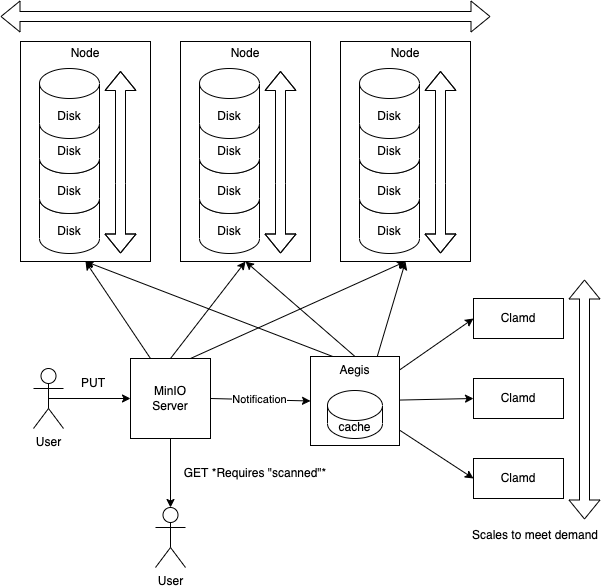
\includegraphics[scale=.4]{diagrams/post-write.png}
  \caption{Post-Write Architecture}
  \label{fig:postWriteArch}
\end{wrapfigure}

This design has many benefits over other potential implementations. Firstly, it
uses the storage provided by MinIO to store all incoming files without having to
manage a separate storage solution. This removes a lot of complexity from the
solution by not having to account for a number of failure conditions that could
occur with a high availability, production ready storage solution. For example,
the solution would not be responsible for handling partial writes, loss of data,
or data corruption. Removing this responsibility allows the solution to focus on
the core functionality of the project, the scanning of files, which is essential
for keeping the project within the time constraints.

Secondly, the design also makes use of the integrated event queue provided by
MinIO. This again removes responsibility from the solution by differing the
scalability and reliability requirements of an event queue to MinIO.

% TODO Design 1: DO THEY KNOW WHAT AEGIS IS?

Lastly, having Aegis dispatch the files to a scalable number of antivirus
scanners allows the solution to scale to meet the demands of the system. This
meets a key requirement as the solution is expected to have the capacity for a
large number of operations. This method does require the use of a load balancer
to effectively distribute the load across the available antivirus scanners.

The design also has a number of drawbacks. Firstly, the design still requires a
small about of cache to temporarily store the object when it is being dispatched
to the antivirus. Provisioning of this cache has to be large enough to handle
the largest file possible to be uploaded to the object store. In reality, this
cache would be provisioned even larger to allow for the temporary storage of
multiple objects while multiple scans are being performed asynchronously. In
addition, the cache needs to be large enough to ensure that the system does not
become overwhelmed by the number of objects being scanned as the system scales.
This is a minor issue as store capacity is cheap and the provisioning of the
cache easy to scale up. Additionally, a higher priority can be given to scaling
up and out antivirus scanners to ensure that the smallest number of files are
being cached, while bring scanned, at any point.

% TODO Design 1: Do they know what get/put is? Do they know distributed storage
% topologies?

The second drawback is that, for each event, Aegis makes a get request for the
object to be scanned. This effectively doubles the number of requests made to
the object store. This also means that Aegis must have the ability to get any
file expected to be scanned and therefore must have access to the whole storage
network. The impact of this drawback is mitigated as the solution is expected to
be deployed on the same network as the object store which should reduce the
latency of each request made by Aegis. However, this still leaves MinIO to
handle twice as many requests with the performance loss being noticed mainly on
more distributed storage topologies.

Thirdly, the design only allows for a single Aegis instance to dispatch all
incoming objects to available scanners. This is a potential bottleneck for the
system as this instance could become overwhelmed by the number of requests it is
receiving. This is a minor issue as the dispatching of objects to scanners is
not as performance intensive as other areas of the solution, such as the actual
scanning, and therefore it is not expected to be a major bottleneck.

Lastly, any object uploaded to the store will have a certain period of time
where it remains unchecked. In this time, the user could potentially download an
unscanned object or the object could cause harm to the store before it is
detected. Although the handling of infected objects is out of scope, in an
actual implementation of the solution, the user could be made unable to download
unscanned objects until they have been scanned.

% TODO Design 1: AWS does this with S3 events 'standard flow'

\subsection*{Design 2 - Upload Queue}
\paragraph{}

% TODO Design 2: More explanation here?
This design created a wrapper around MinIO that the user interacts with instead
of MinIO. This means that all puts go through Aegis before being uploaded to the
object store. The design is shown in figure \ref{fig:uploadQueueArch}.

\begin{wrapfigure}{r}{0.45\textwidth}
  \centering 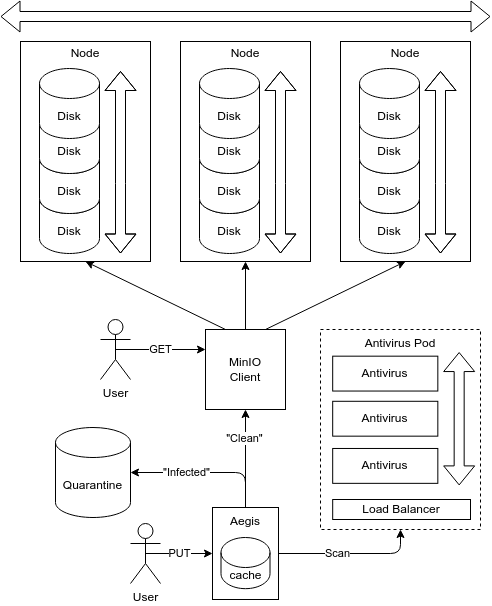
\includegraphics[scale=.4]{diagrams/upload-queue.png}
  \caption{Upload Queue Architecture}
  \label{fig:uploadQueueArch}
\end{wrapfigure}

The main benefit of this design is that the user interacts only with Aegis when
uploading files. This means that all incoming files can be stored within a
temporary storage before ever entering the object store. This offers the best
protection against malicious files as the user cannot ever download an unscanned
or infected file as it is never uploaded to the object store. Infected files can
then either be deleted or moved to a separate quarantine store for analysis.

This designs main advantage also comes with a major drawback. This design
requires Aegis to handle the full throughput of all the puts to the system.
Aegis then has the full responsibility of being available to all puts and, in a
failure scenario, to handle the recovery of the system. Additionally, the cache
provisioned must be large enough to handle the largest files at maximum
throughput with extra room for unexpected delays. This negatively affects the
scope of the project by requiring the solution to prioritise features that are
already covered by MinIO.

% TODO Design 2: Cover mitigation

% TODO Design 2: is this already covered?
Because MinIO is dependent on Aegis to handle the puts, MinIO must wait to be
passed incoming objects sequentially after Aegis has finished processing the
previous object. This removes the potential for aggregate performance where

% TODO Design 2: Talk about how AWS uses this method 'Two Bucket System Flow'

\subsection*{Design 3 - Write Interception}
\paragraph{}

% TODO Design 3: Edit diagram to show quarantine?

Design three is very similar to the second design, however, instead of wrapping
outside the MinIO service, it intercepts the writes from the client before
objects are written to the object store. With this interception, Aegis can scan
the object and decide whether to allow the object to be written to the store or
to quarantine the object. The design is shown in figure
\ref{fig:writeInterceptArch}.

\begin{wrapfigure}{r}{0.4\textwidth}
  \centering 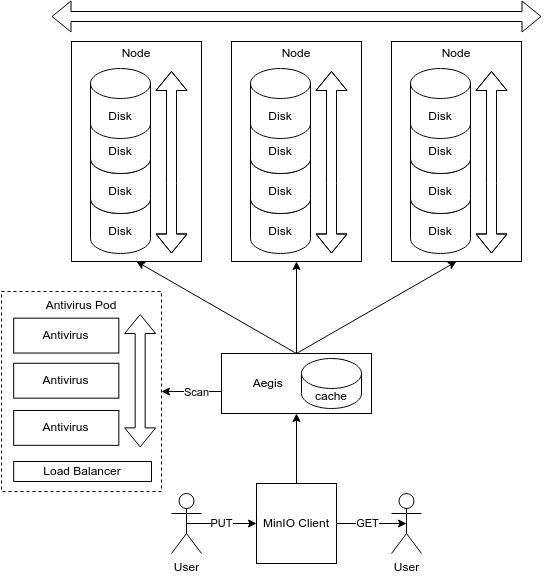
\includegraphics[scale=.3]{diagrams/write-intercept.png}
  \caption{Write Interception Architecture}
  \label{fig:writeInterceptArch}
\end{wrapfigure}

This design has similar benefits as the second design. It offers the most
protection against malicious files by never allowing either unscanned or
infected objects to be stored in the object store. However, it also has similar
drawbacks. This is because Aegis is still in sequence with MinIO meaning that
for optimal throughput, Aegis would need to match the performance of MinIO.

Similar to the upload queue design, this design also requires Aegis to have a
large cache to handle the largest files at maximum throughput. This cache must
also be large enough to handle the number of objects being put by MinIO into the
store. This issue cannot be mitigated without the risk of compromising
performance at increased loads.

However, this design does have an advantage over the second design as there is
less responsibility placed on Aegis to be as failure tolerant. MinIO is still
directly responsible for accepting objects into the store and therefore is still
responsible for the recovery of the system in a failure scenario. This allows
the scope to focus on more related features to malware scanning.

% TODO Design 3: Encrypted???

\subsection*{Design 4 - Per Node}
\paragraph{}

% TODO Design 4: More?
The final design distributes Aegis onto each node in the object store. This
means that each node has a local instance of Aegis that is responsible for
scanning objects before they are written to the store. The design is shown in
figure \ref{fig:perNodeArch}.

\begin{wrapfigure}{r}{0.5\textwidth}
  \centering 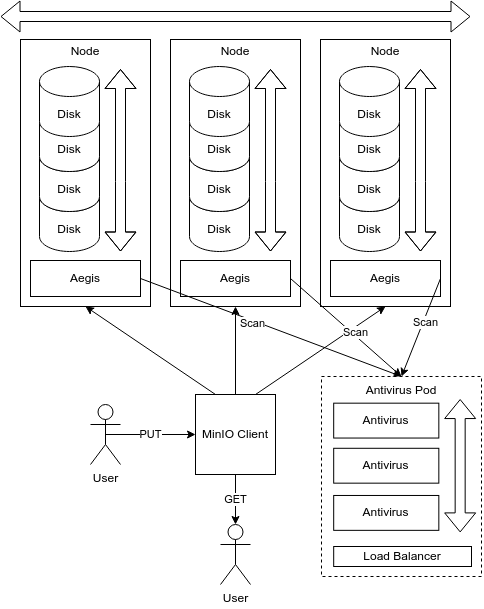
\includegraphics[scale=.3]{diagrams/per-node.png}
  \caption{Antivirus per Node Architecture}
  \label{fig:perNodeArch}
\end{wrapfigure}

This design makes use of the distributed nature of MinIO to match the demand
when scaling out the system. As more nodes are added, more Aegis instances are
added to handle the increased scanning demand. This removes the need for having
a cache repository as Aegis already has access to the files that need scanning.
By removing this single point of failure, in theory, the system only relies on
the antivirus pod to be able to scale out on its own.

Independent scaling of the antivirus pod allow for efficient usage of available
hardware. A simple load based auto-scaler can be used to scale the number of
pods based on the current load. This allows for the system to flexible scale
with the demand of the system and to reduce usage of valuable resources, such as
power. There is also the opportunity to use intelligent scaling techniques to
predict the load on the system and prematurely scale the system to meet the
demand. For example, to scale the number of pods depending on the time of day or
the day of the week.

% TODO Design 4: Explain MinIO terms
The major drawback of this design is that it replies on the ability to scan
whole files by only using data on a single node. In actual implementations,
MinIO makes use of erasure coding to add increased redundancy to the store
\citep{minio-erasure}. Erasure coding splits objects into multiple parts known
as blocks, and then calculates corresponding parity blocks. These data and
parity blocks are then distributed among all nodes in the system allowing for
on-the-fly data recovery even with the loss of multiple drives or nodes . This
means that the Aegis instance on each node only has access to the part available
on their node and therefore will not be able to reconstruct the whole file for
scanning. This makes this design unsuitable for MinIO as it erasure coding is
one of its key features.


\subsection*{Optimal Design}

Given the above evaluations of each design, design one best meets the
requirements and constraints of the project. It makes the most use of the
existing features that MinIO provides in order to handle failure scenarios and
to scale out. This also means that this design has less critical responsibility
and will better fit the scope constraints allowing for more time to be spent on
supplementary features, such as testing, logging, and metric collection. Because
of this, the produced solution will be closer to production-ready than the other
designs.

This design keeps the user in control by giving them the ability to store
unscanned files / known malware without wasting resources on a scan. Protection
can be added per bucket therefore a user could have a known malware bucket and a
clean bucket within the same object store. This allows for the system to be more
flexible and to be able to handle more use cases. Designs two and three would
not be as able to handle this use case as they both scan all objects before they
are written to the store.

The size of the cache required is smaller than all other designs as it only
needs to store the objects actively being scanned. This is in opposition to
upload queue and write interception designs as they have to be prepared to
handle the full demand placed on the store. This makes design one the most
lightweight of all the designs which should lead to a smaller resource
footprint.

% TODO Optimal Design: This is a bad ending :(
Overall, implementing design one is the best option to create a lightweight yet
secure and scalable solution.

\section{Implementation}

% TODO Implementation: What does the final product look like?

\subsection*{Initial Service Creation and
  Configuration} % How I tested each service

% TODO Implementation: Why did I choose to start all the services separately?

Before I started to code the solution, I needed to research, create, configure
and most importantly understand each external service that I would be using. Up
to this point I know what types of services I would need to create, but I did
not know what specific services I would be using. This section will go through
the process of how I chose each service and then initially configured them to
form a bare-bones proof of concept.

\subsubsection*{Object Store - MinIO}
\paragraph{}

The object store is the only service that I did not need to research or compare
as it is already the subject of this project. However; I did need to create and
configure a local instance of MinIO for development. MinIO itself is available
from many sources, including Docker, Homebrew, and the MinIO website. I chose to
use Homebrew, a MacOS package manager, as it is the easiest to install and
update. I then used the MinIO documentation to create a local instance of MinIO
where I can access the web client on \url{http://localhost:9000}. From this I
could create buckets, upload objects to the store and get more familiar with
MinIO's features.

MinIO has integrated the ability to send notifications to event queues depending
on what operation is performed on the store. This makes it quick and easy to set
up a locally running instance of an event queue to read messages sent by MinIO.
MinIO offers wide support for many different event queues, such as Kafka,
Webhook, Redis, PostgreSQL, and many more.

\subsubsection*{Event Queue}
\paragraph{}

Kafka is a popular and well-supported event queue that is used in many different
industries. It offers many features that make it a good choice for this project,
such as high-throughput, low latency and open-source. Kafka is also available
from both Docker and Homebrew make it easy to install and run locally. Most
modern event queues offer similar high throughput and low latency, but Kafka is
lighter in resource usage than other queues, such as RabbitMQ
\citep{kafka-rabbitmq}. This is beneficial as it will be easier to implement and
not over use resources when it has a simple use case.

Kafka has a dependency on Zookeeper, which is a distributed coordination
service. Zookeeper must be installed as a separate service but is available from
the same sources as Kafka. Kafka can be run in Kafka Raft mode (KRaft) which
will eventually replace Zookeeper, but as of writing KRaft has not been fully
adopted yet \citep{kafka-raft}.

With Kafka and Zookeeper setup, I use Kafka's command line interface (CLI) to
start the service and create a topic. I then use the MinIO documentation to
configure MinIO to send all put notifications to the Kafka topic. I can then use
the Kafka CLI to read messages from the topic and see the messages sent by
MinIO. This proves that the event queue is working and that MinIO is sending
messages to it whenever I perform a put operation. An example Kafka message is
available in the appendix in listing \ref{kafka-notif}.

% TODO Event Queue: Reference

\subsubsection*{Antivirus}
\paragraph{}

The antivirus we choose has to meet a list of requirements for it to be suitable
for use in this project. Firstly, it must be able to be scaled with the solution
in order to keep up with the demand placed on the system. Secondly, it must have
a CLI that our program can interact with in order to scan files. Finally, it
must be free or as cheap as possible to make it viable for commercial use. This
narrows down the available options to a few contenders.

Sophos is a popular antivirus that is used by many businesses and is available
for free for personal use, however; is it paid % TODO Antivirus: Sophos

ClamAV however is completely free and open-source. It comes with a scalable and
multi-threaded daemon which can be accessed via CLI for high-performance and
on-demand file scanning. \citep{clamav}. It is capable of scanning many
different file types, including archives and mail files. Build-in is freshclam,
a tool for automatically updating the virus database definitions. The virus
database itself is also open-source and is updated regularly by the open source
community. ClamAV has a docker image and is available from Homebrew.

I have chosen to use ClamAV as it is totally free for commercial use,
open-source and has a CLI that can be used to scan files. It is also very well
documented and has a large community of users. Sophos
% TODO Antivirus: Sophos too expensive

ClamAV comes with a daemon, clamd, that can be run in the background and can be
accessed via a CLI using clamdscan, the clamd client. A configuration file is
needed to point clamdscan to the IP address that the daemon is running. In this
case it is running locally on port 3310. Performing the clamdscan command and
providing a file will scan the file and return the result. An example of this is
available in the appendix in listing \ref{clamd-scan}.

\subsubsection*{Metric Collection}
\paragraph{}

As the project is expected to be as production-ready as possible, a system for
collecting metrics is needed. This will allow the system to monitor its activity
for easier maintenance and debugging. A few different options are available for
metric collection, such as Prometheus, InfluxDB, and Graphite. Each of these

% TODO Metric Collection: Reference why we need metrics TODO Metric Collection:
% Complete comparison

From this comparison, I chose to use Prometheus as it is open-source, uses a
pull model with the option for a push gateway and it does not require a
distributed system to run, unlike InfluxDB. Prometheus is available from both
Docker and Homebrew.

Prometheus is currently unusable as I am not sending it any metrics to collect.
I can still launch the Prometheus server and access the web interface on port
9090. In the meantime I can use the Prometheus documentation to create a
configuration file defining the port and endpoint I expect to be exposing
metrics to, in this case port 2112 and /metrics.

% TODO Metric Collection: Shall I reference Prometheus docs?

\subsubsection*{Audit Log Store}
\paragraph{}

Production-ready software should have a way to store logs for auditing and
analysis purposes. This is a relatively simple requirement as a central database
can be used due to the expected low amount of data needing to be written. The
purpose of the audit log is to store information about the scans performed by
the system with information such as, time and result of the scan as well as the
antivirus used. This gives the system a way to look back at previous scans which
could help with debugging and maintenance.

There are many different options for a database to store the audit logs, such as
PostgreSQL, MySQL, MongoDB, and many more. PostgreSQL remains the most versatile
out of these options as it is a relational database and can be used for many
different purposes. As the use case is simple, keeping to a single database
service is the best option for maintainability and usability. PostgreSQL is also
available from both Docker and Homebrew.

% TODO Audit Log Store: Compare some more databases?

Like Prometheus, PostgreSQL is currently unusable as I am not sending it any
data to store. However, I can still launch the PostgreSQL server and access the
database via PostgreSQL shell prompt (psql). I can create a database and a user
for the database to use. This database can then be exposed to port 5432 on the
localhost ready for Aegis to use.

% TODO Audit Log Store: Reference why we need metrics

\subsubsection*{Data Visualisation}
\paragraph{}

Graphana

% TODO Data Visualisation: Why we need data visualisation TODO Data
% Visualisation: Compare other data visualisation tools - prometheus


% TODO Initial Service: Docker?? Or include that in each service


\subsection*{Aegis}

Now all of the dependencies have been downloaded, initialised and configured,
Aegis can now be coded to interact with them.


The most common language to use for micro-service based projects is GoLang. Go
is a compiled language that is statically typed and high concurrency support.
This makes it a perfect fit for this project to ensure that the system is as
performant as possible. MinIO is also written in Go should allow for easier
integration. Go has certain standards and guidelines for clean architecture that
should be followed to ensure high usability and efficiency.

In Go you should the separate the code into different packages, where each
package represents a distinct function of the system. This allows for easier
maintenance and debugging in the future. These packages are then grouped into
different directories depending on their intended scope. There are three main
directories that are used in GoLang projects, cmd, pkg and internal. The cmd
directory is used to store the main.go file which manages the workflow and is
the entry point of the program. The pkg directory is used to store all of the
packages that are intended to be used by external applications, in this case our
other services. The internal directory is used to store all of the packages that
are intended to be used by the application itself. This is where the packages in
the pkg directory will be consumed to perform the Aegis' core actions as follows:

\begin{itemize}
  \item Listen for PUT events on the event queue
  \item Read the message from the event queue and extract the bucket and object
        path
  \item GET the object from the object store and store in cache
  \item Initiate a scan on the object using the antivirus software
  \item Collect the result of the scan and add tags to the object
  \item Collect metrics throughout the process
  \item Store the result of the scan in the audit log
  \item Expose metrics to Prometheus
\end{itemize}

From these requirements, the internal design of Aegis can be planned. We can
visualise this plan using a class diagram. It is worth noting that Go itself
does not have classed but instead uses structs which can be used to achieve
the same effect. This plan is shown in figure \ref{fig:aegisPlan}.

\begin{wrapfigure}{r}{0.4\textwidth}
  \centering \includegraphics[scale=.3]{diagrams/aegis-plan.png}
  \caption{Plan of Aegis' Internal Packages}
  \label{fig:aegisPlan}
\end{wrapfigure}

This is shown in figure \ref{fig:aegisFileStruct}.
% TODO Aegis: file structure diagram
% TODO Aegis: Class diagram

\begin{wrapfigure}{r}{0.4\textwidth}
  \centering 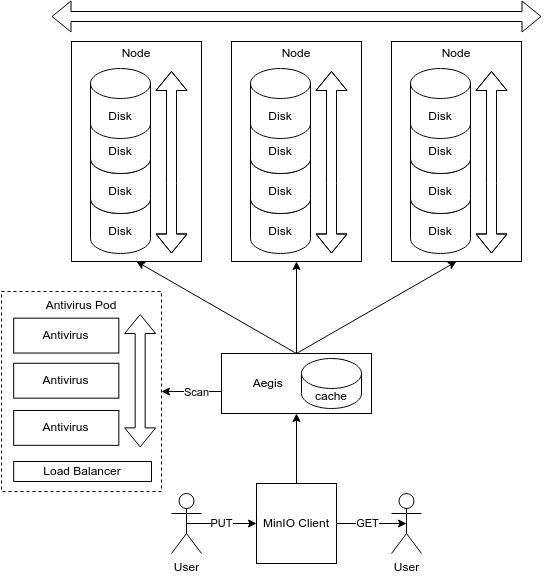
\includegraphics[scale=.3]{diagrams/write-intercept.png}
  \caption{Write Interception Architecture}
  \label{fig:writeInterceptArch}
\end{wrapfigure}

% TODO Aegis: Explain OOP in Go








\subsubsection*{Implementation
  Milestones} % Breakdown of key targets through project

There are many key milestones that can be used to measure the progress of the
project through the duration of its implementation. It is worth noting that
these milestones were created before the implementation of the solution and
therefore are subject to change.

% TODO Milestones: I am talking about a lot of specific things here. Do they
% know what it means?
\begin{itemize}
  \item Setup local antivirus instance
  \item Setup local MinIO instance
  \item Setup local event queue instance
  \item Detect PUT message on Kafka
  \item Read JSON of message to find bucket and object path
  \item Create AV manager service in GoLang
  \item Request GET on Object using message data
  \item Scan Object using Clamd
  \item Act on result of scan - Add tags, result, time and AV used
  \item Configuration file using viper
  \item Add metric collection with Prometheus
  \item Add structured logging with zap
  \item Create Database of Audit Logs with postgresql
  \item Termination of connections to services
  \item Create tests for each package using mockery
  \item Prepare for Kubernetes deployment with k3d
  \item Containerise Aegis with Docker
  \item Automatically configure and start MinIO, Kafka, Clamd, Postgresql,
        Prometheus and Aegis with Helm
  \item Port forward MinIO out of the cluster
  \item Load balancing / performance analysis for Clamd
  \item Expose Postgresql and Prometheus for analytics
  \item Prepare configurations for demo, release etc
  \item Clean-up version control and write readme.me
\end{itemize}

These milestones can be broken down even further into smaller tasks. These are
best represented in Gantt / burndown charts which can be found in the appendix.
% TODO Milestones: Reference


\subsubsection{Code}


\subsection*{Kubernetes Deployment}

\section{Results and Evaluation}
% Evaluate against specification Compare to MinIO Find figures like average scan
% Compare local vs cluster
\subsection*{}

\section{Product Issues / Future work} % What you would do next time
\subsection*{}

\section{Conclusions}
\subsection*{}

\section{Reflection on Learning} % Fuck knows
\subsection*{}

\section{Appendix}
% TODO Appendix: Add figues and tables to appendix
%
%
%
\lstinputlisting[frame=single, caption={Example Kafka Notification},
label=kafka-notif, numbers=left]{assets/example-notif.json}

\lstinputlisting[frame=single, caption={Example Kafka Notification},
label=clamd-scan, numbers=left]{assets/example-clamd-scan.txt}

\bibliographystyle{cardiff} \bibliography{references}

\end{document}

% TEMPLATED
% \begin{figure}[!ht]
%   \centering \includegraphics[scale=.55]{assets/extracred}
%   \caption{Bouncing and pitching motion as a function of time}
%   \label{fig:bounceAndPitch}
% \end{figure}

% \begin{table}[!ht]
%   \begin{center}
%     \caption{Calculated values}
%     \label{tab:calculated}
%     \begin{tabular}{|c|c|}
%       \hline
%     \end{tabular}
%   \end{center}
% \end{table}

% Appendix \onecolumn \textwidth=456pt \paperwidth=577pt \hoffset=-30pt
% \newpage
% \newpage
% \clearpage


% \pagestyle{headings}
% \section{Appendix A}
% \centering Heading \footnotesize

% \normalsize

% \csvautolongtable{assets/vibProj.csv}
%
